\documentclass[tikz,border=10pt]{standalone}
\usepackage{tikz}

\begin{document}

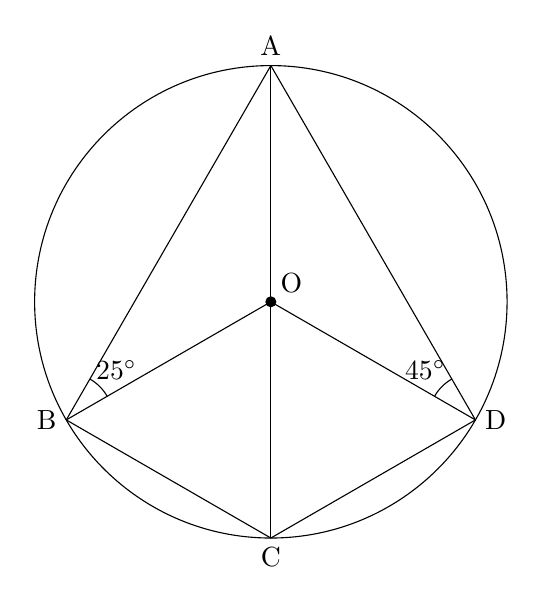
\begin{tikzpicture}[scale=1]
    % Define the circle with center O and radius
    \coordinate (O) at (0,0);
    \draw (O) circle (3cm);

    % Define the points on the circle based on the image's layout
    \coordinate (A) at (90:3cm);   % Top point
    \coordinate (B) at (210:3cm);  % Bottom-left point
    \coordinate (C) at (270:3cm);  % Bottom point
    \coordinate (D) at (330:3cm);  % Bottom-right point

    % Draw the lines connecting the points
    \draw (A) -- (B);
    \draw (B) -- (C);
    \draw (C) -- (D);
    \draw (D) -- (A);

    % Draw the radial lines from center O
    \draw (O) -- (A);
    \draw (O) -- (B);
    \draw (O) -- (C);
    \draw (O) -- (D);

    % Draw the labels for the points
    \node [above] at (A) {A};
    \node [left] at (B) {B};
    \node [below] at (C) {C};
    \node [right] at (D) {D};
    \node [above right] at (O) {O};

    % Draw a small dot for the center O
    \fill (O) circle (2pt);

    % Draw the angle arcs and values
    % Angle at B (between BA and BO)
    \draw (B) + (30:0.6) arc (30:60:0.6);
    \node at ([shift={(45:0.9)}]B) {$25^{\circ}$};

    % Angle at D (between DA and DO)
    \draw (D) + (120:0.6) arc (120:150:0.6);
    \node at ([shift={(135:0.9)}]D) {$45^{\circ}$};

\end{tikzpicture}

\end{document}
